\documentclass[a4paper,12pt]{article}

% ================================================== DATOS ==================================================

% Información de la materia
\newcommand{\codMateria}{TA138}
\newcommand{\nombreMateria}{Taller de Diseño de}
\newcommand{\cuatrimestre}{1.\textsuperscript{er} Cuatrimestre}

% Información del TP
\newcommand{\TpTitulo}{Proyecto Integrador -- Checkpoint 1}
\newcommand{\fecha}{\today}
\newcommand{\group}{Grupo 5}

% Información de alumnos
\newcommand{\nombreA}{Lautaro García Vitale}
\newcommand{\padronA}{110028}
\newcommand{\emailA}{lagarciav@fi.uba.ar}

\newcommand{\nombreB}{Santiago Manuel Cabrera}
\newcommand{\padronB}{110445}
\newcommand{\emailB}{smcabrera@fi.uba.ar}

\newcommand{\nombreC}{Francisco Javier Moya}
\newcommand{\padronC}{109899}
\newcommand{\emailC}{fjmoya@fi.uba.ar}

% ================================================== PAQUETES =================================================

% Codificación y lenguaje
\usepackage[utf8]{inputenc}
\usepackage[ddmmyy]{datetime}
\usepackage[language=spanish]{lipsum}
\usepackage[spanish]{datetime2}
\usepackage[T1]{fontenc}
\usepackage[spanish,es-nodecimaldot]{babel}
\usepackage[a4paper,margin=2.5cm]{geometry}
\usepackage{amsmath,amssymb,amsthm,mathtools}
\usepackage{bm}
\usepackage{physics}
\usepackage{setspace}
\usepackage{hyperref}
\usepackage{enumitem}

% Márgenes y página
\usepackage{geometry}
\usepackage{fancyhdr}
\usepackage{emptypage}
\usepackage{parskip}

% Encabezado personalizado
\pagestyle{fancy}
\fancyhf{}
\rhead{\group}
\lhead{\TpTitulo}
\cfoot{\thepage}

% Tipografía matemática
\usepackage{mathtools}
\usepackage{amssymb}
\usepackage{amsfonts}
\usepackage{amsthm}
\usepackage{yhmath}
\usepackage{dsfont}
\usepackage{esdiff}
\usepackage{xfrac}
\usepackage{siunitx}
\sisetup{per-mode=reciprocal, separate-uncertainty=true}

% Gráficos y tablas
\usepackage{graphicx}
\usepackage{float}
\usepackage{booktabs}
\usepackage{caption}
\usepackage{subcaption}
\usepackage{multirow}
\usepackage{adjustbox}

% TikZ y gráficos avanzados
\usepackage{pgfplots}
\pgfplotsset{compat=1.18}
\usepackage{tikz}

% Código fuente y resaltado
\usepackage{minted}
\usepackage{tcolorbox}
\definecolor{codebg}{rgb}{0.95,0.95,0.95}  % Color de fondo del código
\usemintedstyle{friendly}                  % Estilo del resaltado de sintaxis
\setminted{
    linenos=true,                          % Numeración de líneas
    bgcolor=codebg,                        % Color de fondo del código
    fontsize=\footnotesize,                % Tamaño de la fuente
    frame=lines,                           % Estilo del marco
    framesep=2mm,                          % Separación del marco
    baselinestretch=1.2,                   % Espaciado entre líneas
    breaklines=true,                       % Romper líneas largas automáticamente
    encoding=utf8,                         % Codificación del archivo
    tabsize=4,                             % Tamaño de la tabulación
}

% Misceláneo
\usepackage{anyfontsize}
\usepackage{xcolor}
\usepackage{url}
\usepackage{comment}
\usepackage{multicol}
\usepackage[numbers,square]{natbib}

% Estilo de bibliografía
\bibliographystyle{IEEEtran}


% ==============================================================================================================
% ==============================================================================================================


\begin{document}

% ================================================== CARÁTULA ==================================================

\pagenumbering{arabic} % Comienza la numeración

\vspace{-1 cm} % La primera hoja tiene que tener menos espaciado

\begin{center}
  \begin{minipage}{0.8 cm}
    
\includegraphics[width=\linewidth]{img/fiuba.png}
  \end{minipage}
  \begin{minipage}{\widthof{\large{\textsc{Universidad de Buenos Aires}}}}
    \centering
    \large{\textsc{Universidad de Buenos Aires}}\\
    \large{\textsc{Facultad de Ingeniería}}\\
    \small{Año 2026 -- \cuatrimestre}
  \end{minipage}
\end{center}
\vspace{10mm}
\begin{center}
  \huge{\underline{\textsc{\nombreMateria}}} \\
  \huge{\underline{\textsc{Circuitos Electrónicos}}} \\
  \vspace{7 pt}
  \Large{\TpTitulo \\}
  \vspace{3mm}
  \large{\group}
\end{center}

\newcommand{\anchopadron}{\widthof{000 000}}
\begin{center}
  \begin{tabular}{l l l}
    \nombreA & \parbox{\anchopadron}{\raggedleft \padronA} & \emailA \\
    \nombreB & \parbox{\anchopadron}{\raggedleft \padronB} & \emailB \\
    \nombreC & \parbox{\anchopadron}{\raggedleft \padronC} & \emailC 
  \end{tabular}
\end{center}
\vspace{8mm}

\begin{center}
\renewcommand{\arraystretch}{1.3}
\begin{tabular}{@{}r p{0.62\textwidth}@{}}
\textbf{Tutor:} & Federico Gabriel D'Angiolo. \\ 
\textbf{Docentes:} & Julio Guillermo Zola, Marcelo Adrián Bruno, Sergio Quinteros y Juan Guido Salaya.
\end{tabular}
\end{center}

\vspace{2em}
\thispagestyle{empty}

\begin{abstract}
El presente informe corresponde al primer \textit{checkpoint} del proyecto integrador, centrado en el diseño y análisis del regulador lineal de una fuente de alimentación destinada a aplicaciones industriales y automotrices. En esta etapa se aborda el desarrollo del regulador LDO (\textit{Low Drop Out}) encargado de generar una tensión de salida estable de 5 V a partir de una tensión intermedia de aproximadamente 9,5 V, proveniente de una etapa conmutada previamente definida a nivel conceptual.

Se estudiarán en detalle las decisiones de diseño del amplificador de error y del transistor de paso, así como la implementación de los lazos de realimentación de tensión y de corriente. En particular, se incorporará un mecanismo de protección por sobrecorriente con característica \textit{foldback}, orientado a mejorar la robustez del sistema frente a condiciones de falla.

El diseño propuesto será validado mediante simulaciones, evaluando parámetros clave como la ganancia de lazo, la regulación de línea y de carga, y el comportamiento de la protección. De este modo, se buscará establecer una base sólida para las etapas posteriores del proyecto, que contemplan la implementación física e integración completa del sistema de alimentación.
\end{abstract}

\newpage

\tableofcontents

\newpage

\section{Introducción}

El diseño de sistemas de alimentación eficientes y robustos constituye un aspecto fundamental en aplicaciones electrónicas modernas, particularmente en entornos industriales y automotrices, donde las condiciones de operación pueden variar significativamente. En este contexto, el presente trabajo aborda el desarrollo de una fuente de alimentación capaz de generar una tensión de salida de $\SI{5}{\volt}$ ($V_O$), adecuada para alimentar dispositivos sensibles como microcontroladores, sensores y módulos de comunicación, a partir de una fuente de entrada proveniente de una batería con un rango amplio de variación, comprendido entre $\SI{12}{\volt}$ y $\SI{30}{\volt}$ ($V_\text{IN}$).

Con el objetivo de alcanzar altos niveles de eficiencia sin comprometer la calidad de la señal de salida, se adopta una arquitectura de regulación en dos etapas. En primer lugar, se emplea un convertidor conmutado tipo \textit{buck} que reduce la tensión de entrada a un nivel intermedio cercano a $\SI{9,5}{\volt}$ ($V_\text{REG}$), permitiendo disminuir las pérdidas de potencia asociadas. Posteriormente, una etapa lineal de bajo \textit{dropout} (LDO) se encarga de estabilizar la tensión final en $\SI{5}{\volt}$, proporcionando una salida con bajo nivel de \textit{ripple} y adecuada regulación frente a perturbaciones. Todo esto se representa en la Figura \ref{fig:proyecto}.

\begin{figure}[H]
  \centering
  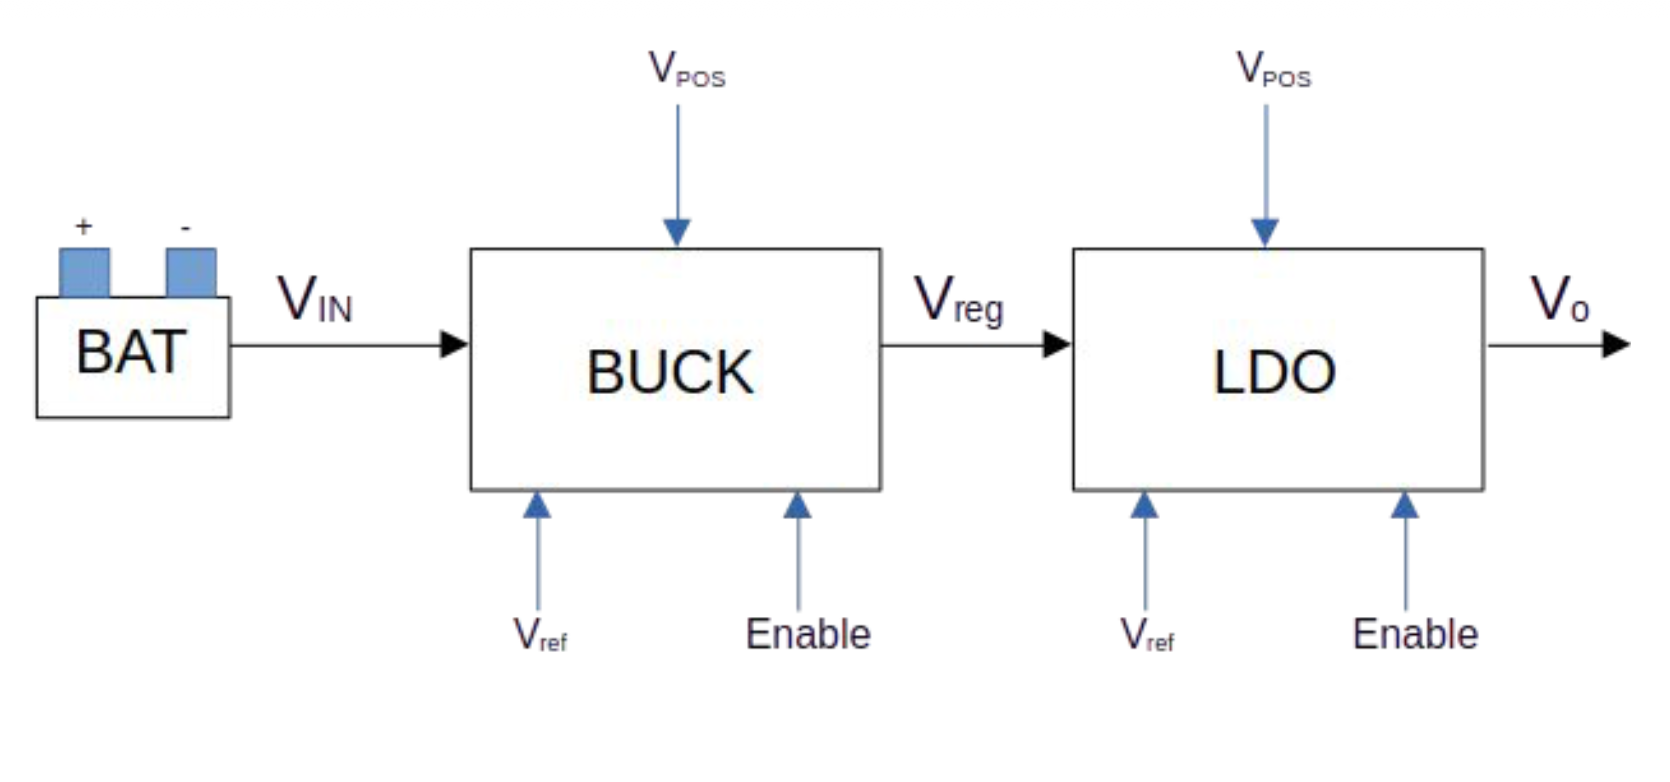
\includegraphics[scale=0.33]{img/proyecto.png}
  \caption{Proyecto Integrador.}
  \label{fig:proyecto}
\end{figure}

El desarrollo del proyecto se encuentra estructurado en distintas etapas, siguiendo una metodología de diseño que abarca desde la definición conceptual hasta la validación experimental. En particular, el presente informe corresponde al primer \textit{checkpoint}, centrado en el diseño del regulador lineal. 

En esta instancia se abordan aspectos clave como la selección del transistor de paso (considerando restricciones de caída de tensión, disipación térmica y capacidad de corriente) así como el diseño de los lazos de control en régimen estático.

Asimismo, se analiza el comportamiento del lazo de regulación de tensión, con el fin de garantizar que la salida permanezca dentro del margen especificado de $(5{,}0 \pm 0{,}1)\ \text{V}$ ante variaciones de carga y de tensión de entrada. De manera complementaria, se desarrolla el lazo de control de corriente orientado a la protección del sistema, incluyendo la implementación de un mecanismo de limitación y reducción progresiva de corriente (\textit{foldback}), que resulta crítico frente a condiciones de sobrecarga o cortocircuito.

Finalmente, se validan mediante simulación las prestaciones del diseño propuesto, verificando el cumplimiento de las especificaciones eléctricas establecidas, como paso previo a etapas posteriores de implementación física e integración en PCB. Este enfoque permite asegurar la viabilidad del sistema antes de avanzar hacia instancias de mayor complejidad dentro del desarrollo del proyecto.

\section{Diseño teórico}

A continuación se detallan las decisiones de diseño empleadas para el regulador lineal LDO.

\subsection{Amplificador de error y transistor de paso}

El funcionamiento de un regulador lineal tipo LDO se basa fundamentalmente en la interacción entre dos bloques esenciales: el transistor de paso y el amplificador de error. El primero actúa como elemento de control de potencia, modulando su conducción de manera continua para ajustar la tensión aplicada a la carga. El segundo, por su parte, es el encargado de comparar la tensión de salida con una referencia estable y generar la señal de control adecuada para gobernar al transistor de paso.

En este contexto, la utilización de un amplificador diferencial resulta particularmente conveniente. Este tipo de configuración permite comparar directamente la tensión de salida con una referencia fija, ofreciendo una alta ganancia diferencial. Además, presentan un mejor rechazo al modo común y una mayor estabilidad térmica, características deseables en sistemas de regulación de precisión.

Dado que la referencia utilizada es de continua ($V_\text{ref}$), el amplificador de error opera también en régimen de continua. Esto implica que no es necesario procesar señales alternas ni excursiones negativas significativas, lo que permite simplificar el diseño prescindiendo de un riel de alimentación negativo. De esta manera, el circuito puede implementarse utilizando únicamente una alimentación positiva ---que en este caso será $V_\text{REG}$---, lo cual resulta ventajoso en términos de complejidad, consumo y compatibilidad con el resto del sistema. 

El hecho de utilizar un transistor PNP como transistor de paso, ubicado en la rama alta del regulador, permite obtener una baja tensión de \textit{dropout}, ya que su conducción se controla reduciendo la tensión de base respecto del emisor, sin necesidad de generar niveles de excitación superiores a la tensión de entrada. Esto facilita que el transistor opere cercano a saturación cuando el regulador se aproxima a su límite, minimizando la caída de tensión entre entrada y salida. En contraposición, configuraciones basadas en transistores NPN o MOSFET en posiciones equivalentes requieren mayores tensiones de excitación, lo que incrementa la caída mínima alcanzable.

En este contexto, la utilización de una estructura cuasi-darlington resulta particularmente adecuada, ya que permite incrementar significativamente la ganancia de corriente efectiva de la etapa de salida sin introducir penalizaciones significativas en la tensión de \textit{dropout}. En particular, el transistor NPN del cuasi-darlington actúa como etapa excitadora, suministrando la corriente necesaria para polarizar la base del transistor de paso. De este modo, el amplificador de error no necesita entregar directamente la corriente de base requerida por el transistor de potencia, lo que reduce su carga y simplifica su diseño.

Además, esta configuración mejora el comportamiento del regulador frente a variaciones de carga, ya que disminuye la dependencia del funcionamiento global respecto de la ganancia en corriente (\(\beta\)) del transistor de paso, la cual puede variar considerablemente con la corriente y la temperatura. Al aumentar la ganancia efectiva del conjunto, se logra una respuesta más robusta y predecible.

De este modo, el diseño preliminar se muestra en la Figura \ref{fig:circuito1}.

\begin{figure}[H]
  \centering
  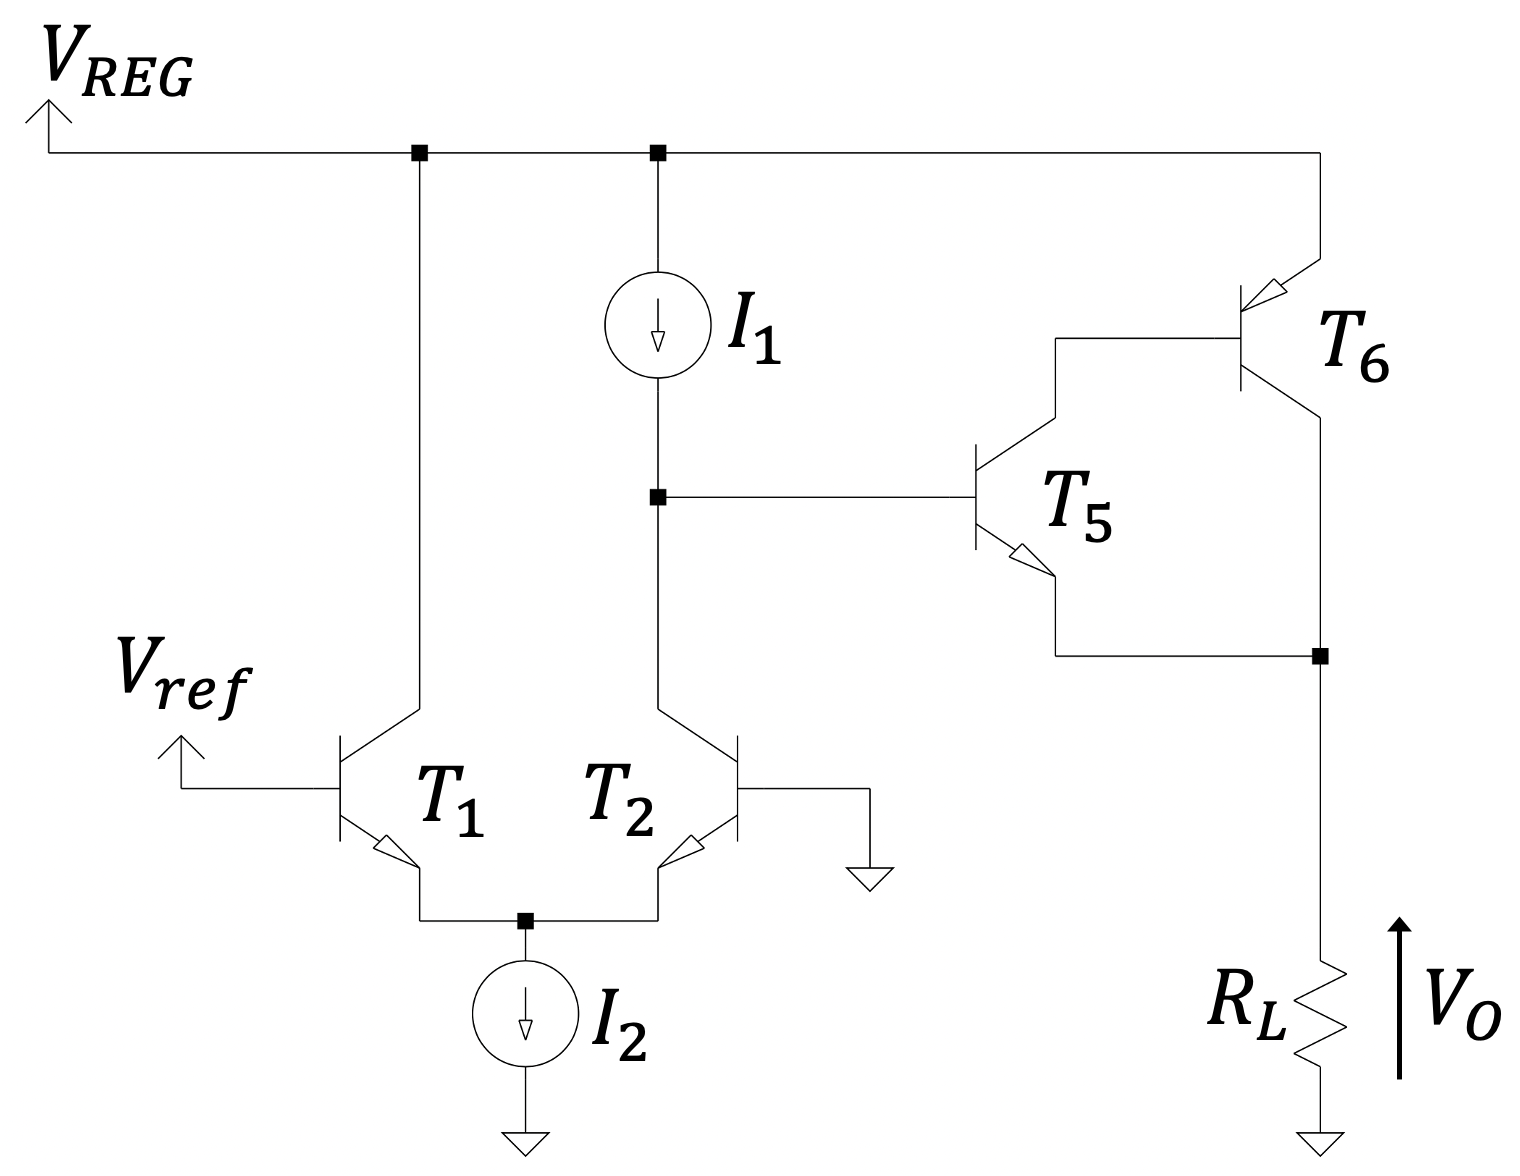
\includegraphics[scale=0.33]{img/circuito1.png}
  \caption{Circuito preliminar.}
  \label{fig:circuito1}
\end{figure}

La elección de una carga activa permite obtener ganancias elevadas necesarias para el correcto funcionamiento del lazo de tensión. Se escogieron fuentes espejo simples por sobre otras configuraciones ya que estas son menos susceptibles a variaciones de temperatura, por lo que la corriente de polarización va a ser más estable. Además, se agregaron resistores para aumentar la ganancia y balancear las ramas si llegase a haber un desapareamiento en las mismas. Estos cambios se muestran en la Figura \ref{fig:circuito2}.

\begin{figure}[H]
  \centering
  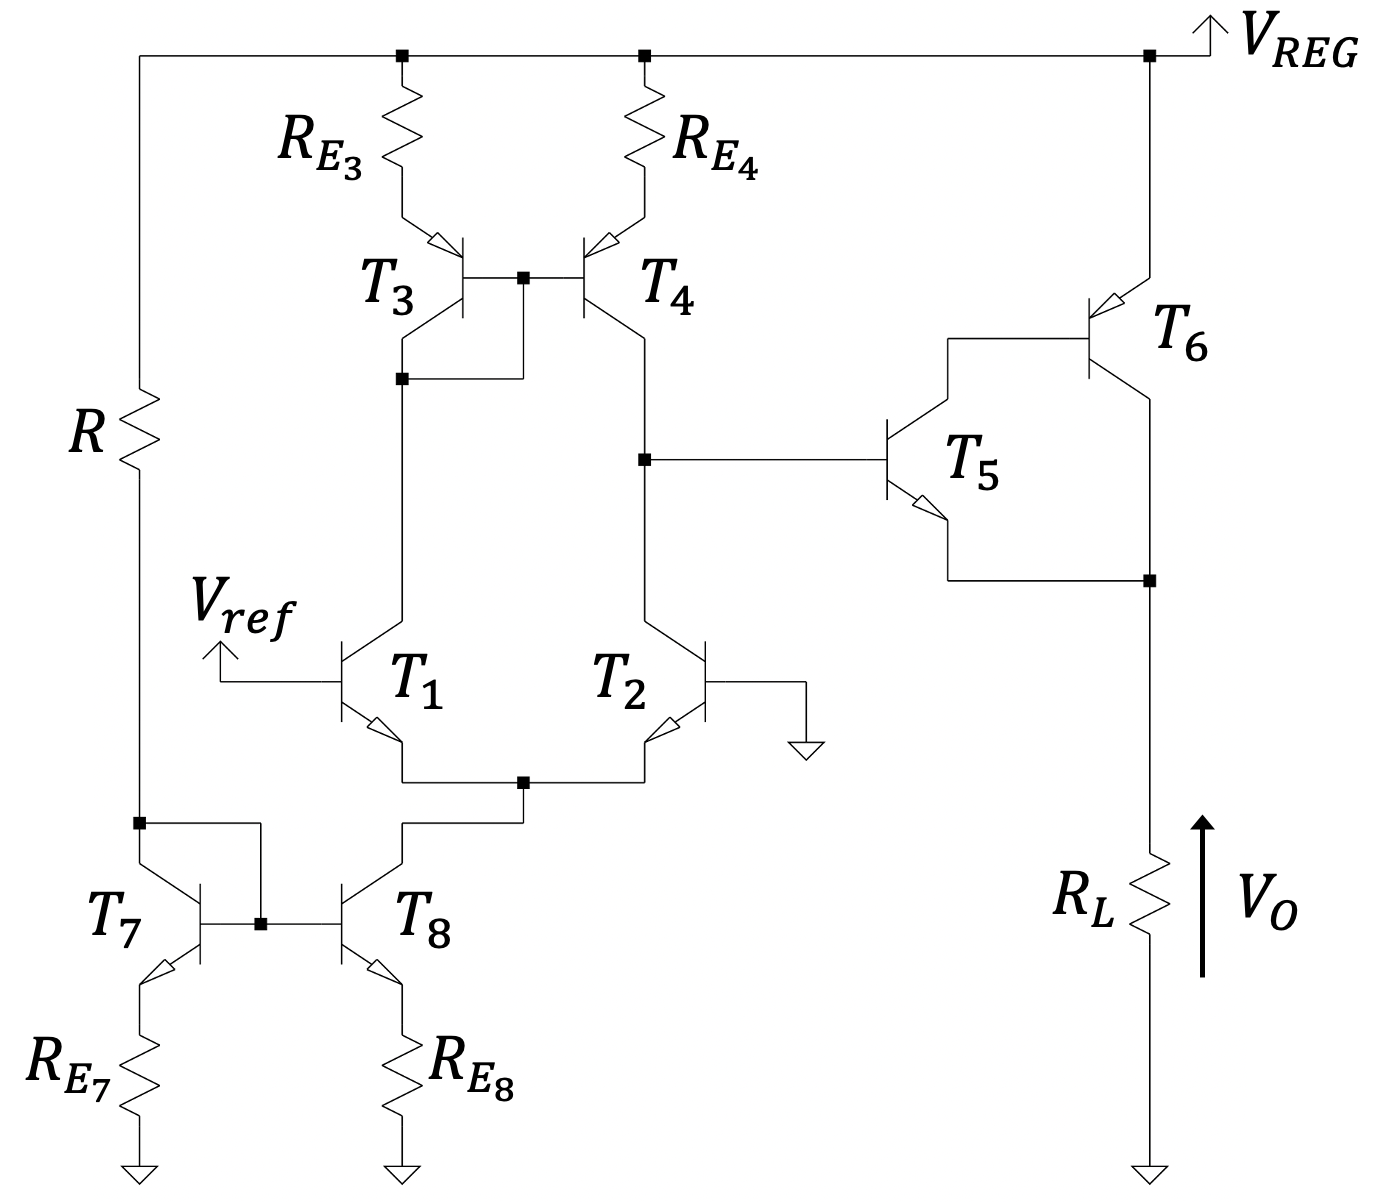
\includegraphics[scale=0.43]{img/circuito2.png}
  \caption{Circuito a lazo abierto.}
  \label{fig:circuito2}
\end{figure}

Para el transistor de paso $T_6$ se eligió el TIP32, ya que es un dispositivo de potencia capaz de manejar una corriente de colector continua de hasta $\SI{3,0}{\ampere}$, cumpliendo con margen el requerimiento de $I_{max} = \SI{1,5}{\ampere}$. Además, soporta una tensión colector-emisor máxima de $\SI{40}{\volt}$ y viene en encapsulado TO-220AB, lo que facilita la disipación térmica en aplicaciones de regulación lineal, pudiendo manejar potencias de hasta $\SI{40}{\watt}$ a $T_C = \SI{25}{\celsius}$. Para el resto de los transistores, se escogieron los BC547 y BC557 según si son NPN o PNP, respectivamente, por su amplia disponibilidad, sus parámetros adecuados para aplicaciones de señal y por tratarse de dispositivos \textit{through-hole} (de montaje pasante), lo que facilita su implementación al no requerir tecnología SMD.

Como elemento de referencia de tensión se emplea un TL431, dispositivo de tres terminales ajustable, configurado para proporcionar una tensión de $\SI{2,5}{\volt}$. La elección de este valor no es arbitraria: por un lado, permite establecer un punto de operación adecuado para el par diferencial sin exceder la tensión de salida disponible, y por otro, resulta conveniente al ser un submúltiplo de la tensión de salida deseada, simplificando el diseño del lazo de realimentación.

En particular, al trabajar con una referencia de $\SI{2,5}{\volt}$, la obtención de la tensión de salida puede lograrse mediante un divisor resistivo formado por dos resistencias iguales, lo que reduce la sensibilidad a desajustes y dispersiones tecnológicas, especialmente si ambas provienen de la misma tirada de fabricación.

Adicionalmente, este nivel de referencia garantiza que el transistor \(T_8\) opere en modo activo directo. En efecto, la tensión aplicada a su base resulta suficiente para polarizar la juntura base-emisor en directa, permitiendo que conduzca corriente de manera controlada y asegurando así el correcto funcionamiento de la fuente de corriente que alimenta al par diferencial.

\begin{figure}[H]
  \centering
  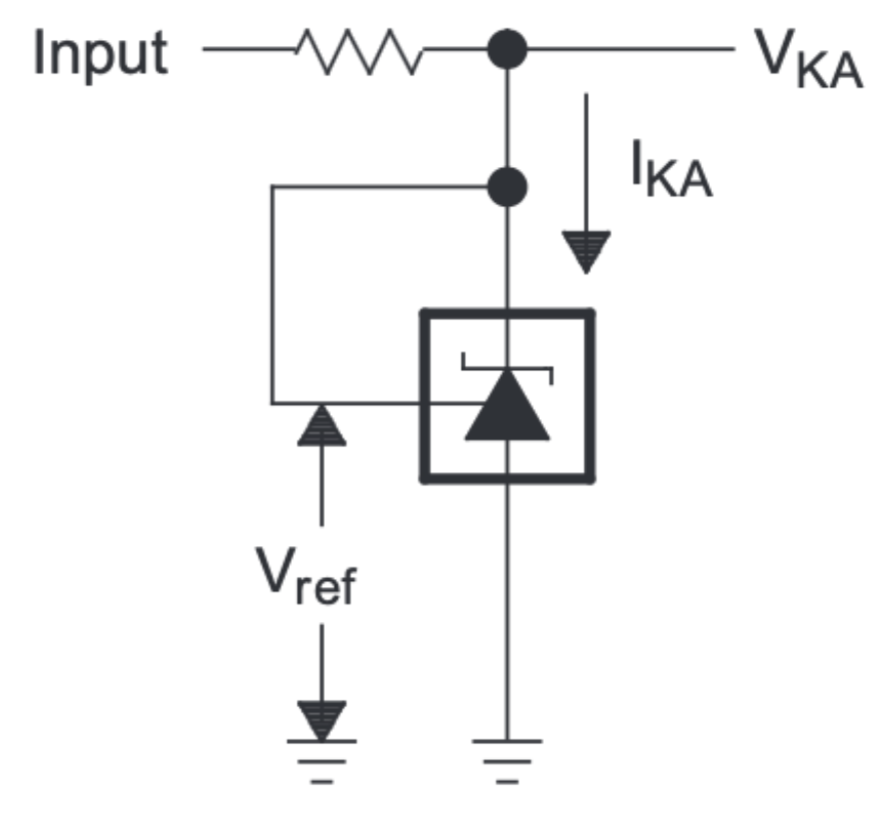
\includegraphics[scale=0.33]{img/referencia.png}
  \caption{Tensión de referencia implementada.}
  \label{fig:referencia}
\end{figure}

En la Figura 4 se presenta el modelo de referencia adoptado para el TL431. En esta configuración, la terminal etiquetada como \textit{Input} corresponde a la tensión de alimentación \(V_\text{REG}\), mientras que la tensión entre cátodo y ánodo cumple \(V_{KA} = V_\text{ref}\), fijando así el punto de operación del dispositivo.

De acuerdo con la hoja de datos del TL431, la tensión de referencia presenta un valor típico de \(V_\text{ref} = 2{,}495\,\text{V}\), con un rango comprendido entre \(2{,}483\,\text{V}\) y \(2{,}507\,\text{V}\), especificado para una corriente de cátodo $I_{KA} = \SI{10}{\milli\ampere}$. Este valor de corriente no es arbitrario, ya que garantiza que el dispositivo opere en su región de regulación con buena precisión.

En este contexto, la resistencia de cátodo ($R_K$) se elige de \(680\,\Omega\) con el objetivo de establecer una corriente de cátodo del orden de los \(10\,\text{mA}\), pues la corriente que circula puede aproximarse como
\[
I_{KA} \approx \frac{V_\text{REG} - V_\text{ref}}{R_K} = \frac{9,5\,\text{V} - 2,5\,\text{V}}{680\,\Omega} \approx 10,3\,\text{mA}.
\]

Nótese que al querer calcular el valor de la resistencia de polarización $R$ ---ver Figura \ref{fig:circuito2}---, se observa una alta influencia de la carga $R_L$ en el mismo ---véase Apéndice A---, por lo que se deberá realimentar negativamente el circuito implementando un lazo de tensión para disminuir dicha influencia.

La implementación de realimentación negativa no solo reduce la dependencia respecto de la carga, sino que además mejora la precisión de la tensión de salida, disminuye la sensibilidad a variaciones de parámetros y perturbaciones, y contribuye a estabilizar el punto de operación del circuito.

\subsection{Lazo de tensión}

El esquema del lazo de realimentación propuesto consiste en muestrear la tensión de salida y sumar tensión a la entrada del amplificador (MVSV). El diagrama en bloques se muestra en la Figura \ref{fig:bloques}, donde $a$ es la ganancia a lazo abierto y $f$ es la ganancia del realimentador.

\begin{figure}[H]
  \centering
  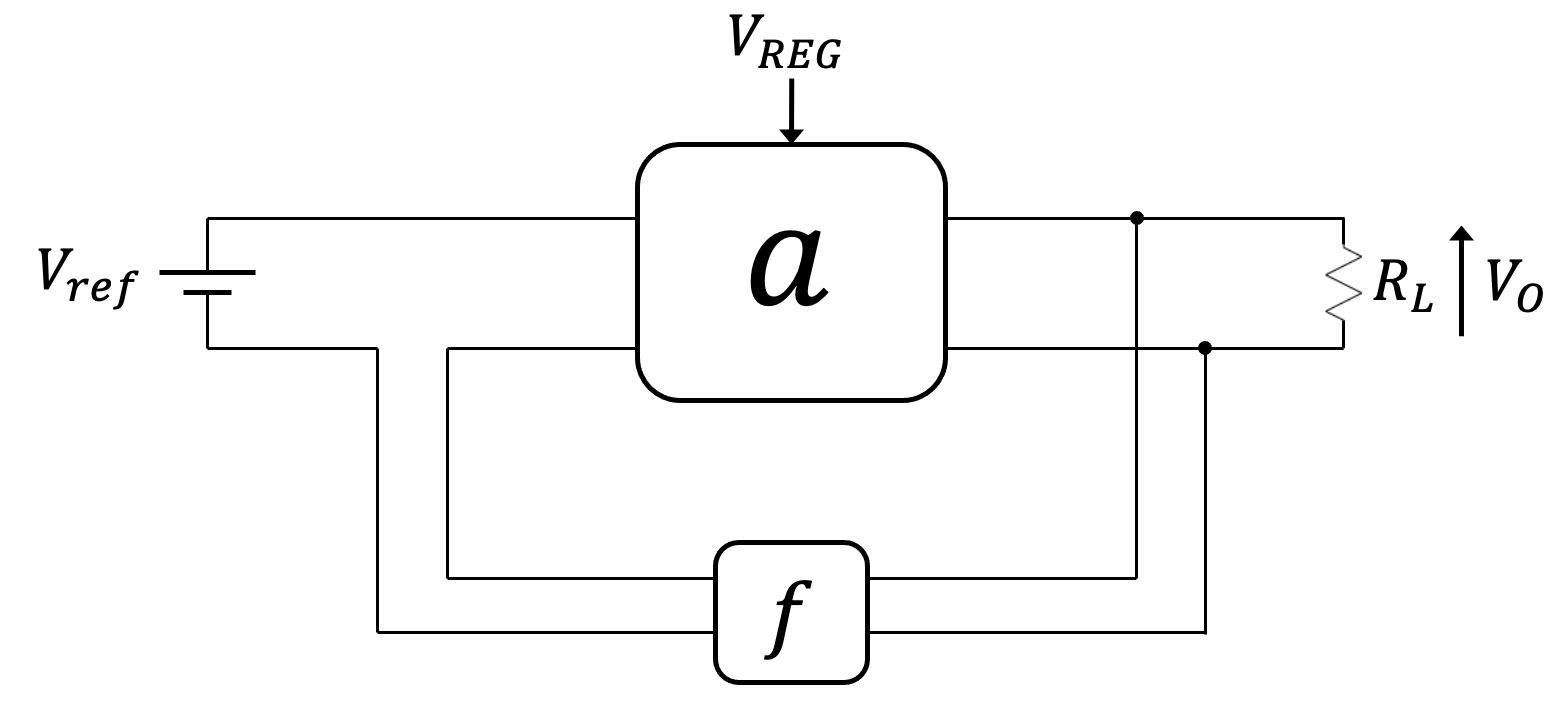
\includegraphics[scale=0.33]{img/bloques.png}
  \caption{Diagrama en bloques del circuito realimentado.}
  \label{fig:bloques}
\end{figure}

De este modo, la ganancia a lazo cerrado $A$ es $V_O / V_\text{ref} = 2$ y verifica 

\begin{equation}
    A = \frac{a}{1+af}.    
    \label{eq:ganancia lazo cerrado}
\end{equation}



Si la ganancia de lazo $T = af$ es muy elevada, entonces $A \approx 1/f$, por lo que $f = 1/2$.

Como se mencionó en la sección anterior, se propone un divisor resistivo como bloque realimentador, de froma tal que 

\[
f = \frac{R_2}{R_1 + R_2}.
\]

Esto se verifica si $R_1 = R_2$ y se escogió el valor de 10 k$\Omega$. En la Figura \ref{fig:circuito3} se observa el circuito a lazo cerrado.

\begin{figure}[H]
  \centering
  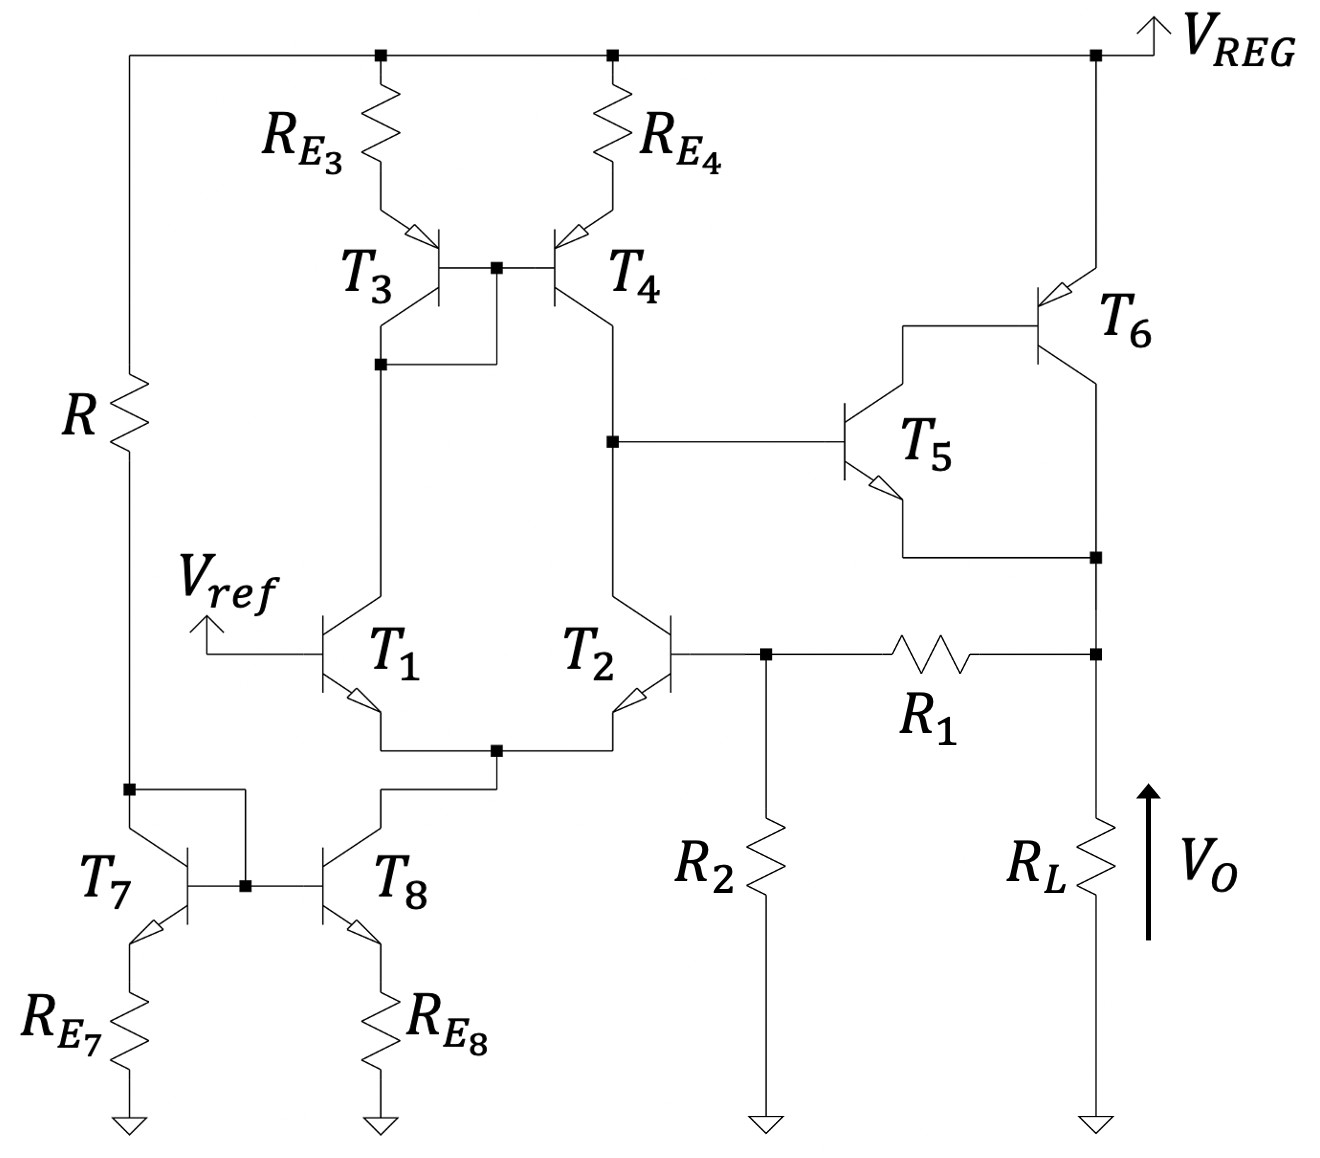
\includegraphics[scale=0.43]{img/circuito3.png}
  \caption{Circuito a lazo cerrado.}
  \label{fig:circuito3}
\end{figure}

Suponiendo que por cada rama del par diferencial circula una corriente de 1 mA, entonces por la resistencia $R$ circulará una corriente de aproximadamente 2 mA. Despreciando la caída de tensión en los resistores de emisor, se tiene que $R = I_R (V_\text{REG} - V_{{BE}_7})$, donde $V_{{BE}_7} \approx 0,7$ V y $V_\text{REG} = (9,5 \pm 0,2)$ V. Teniendo en cuenta los valores comerciales, se obtiene $R = 4,7\,\text{k}\Omega$.

\subsection{Lazo de corriente}

Con el objetivo de proteger la carga ante un posible cortocircuito, al circuito de la \autoref{fig:circuito3} se le añadirá un lazo de corriente. El mismo será de tipo \textit{foldback}, por lo que tendrá la característica se muestra en la Figura \ref{fig:curva_foldback}.

\begin{figure}[H]
  \centering
  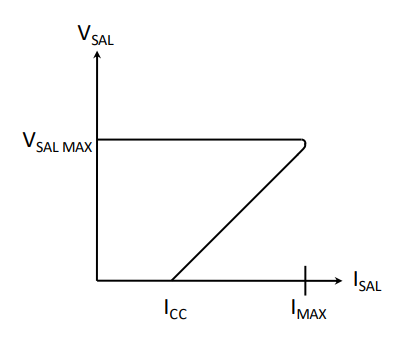
\includegraphics[scale=0.6]{img/Curva_foldback.png}
  \caption{Curva del \textit{foldback}.}
  \label{fig:curva_foldback}
\end{figure}

En este proyecto se buscará $I_{CC} = 0,4 \, \text{A}$ y que $I_{\text{MAX}} = 1,5 \, \text{A}$. 

Se propusieron dos diseños para el lazo de corriente: el primero consiste en una serie de amplificadores diferenciales implementados con OpAmps. El mismo resultaba excesivamente complejo, ya que requería de 5 amplificadores. Por ello, se optó por el segundo diseño, que implementa un circuito equivalente, pero con un solo OpAmp en configuración sumador.

\subsubsection{Primer diseño}

El circuito de la Figura \autoref{fig:circuito3} se modifica como se muestra en la Figura \ref{fig:Lazo de corriente 1}.

\begin{figure}[H]
  \centering
  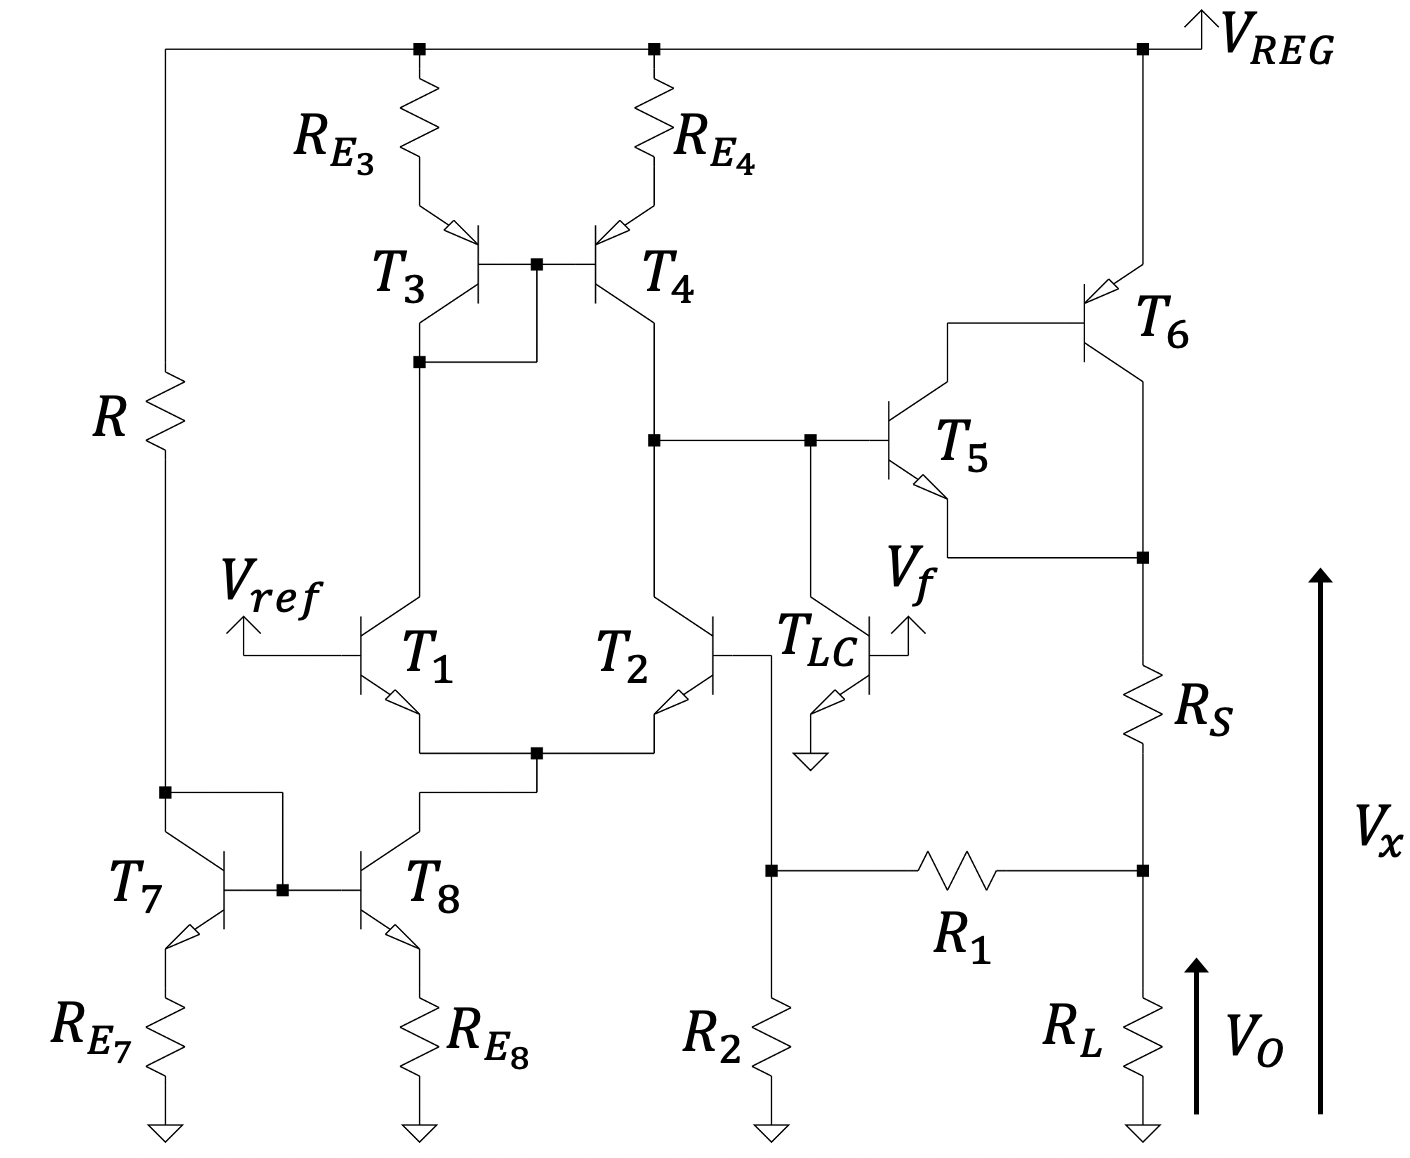
\includegraphics[scale=0.4]{img/circuito4.png}
  \caption{Circuito con lazo de corriente.}
  \label{fig:Lazo de corriente 1}
\end{figure}

Cabe destacar que se añadieron la resistencia $R_S$, el transistor $T_\text{LC}$ y los nodos $V_{\text{x}}$ y $V_{\text{f}}$. También se agregó el bloque representado en la Figura \ref{fig:Lazo de corriente 2}.

\begin{figure}[H]
  \centering
  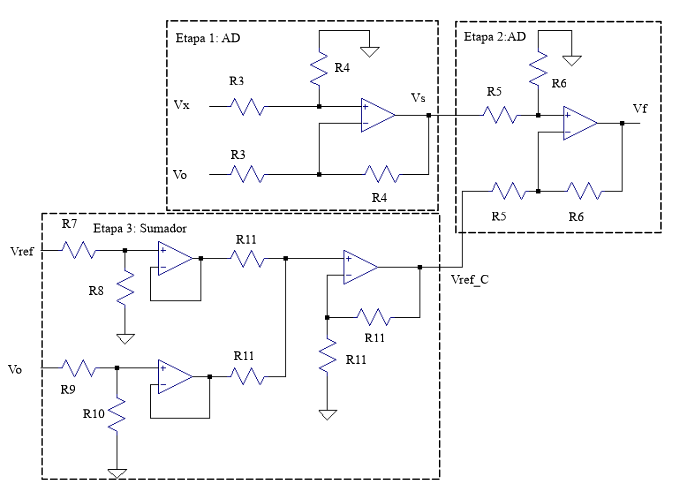
\includegraphics[scale=0.65]{img/Lazo de Corriente 2(Bloque).png}
  \caption{Bloque del lazo de corriente}
  \label{fig:Lazo de corriente 2}
\end{figure}

El mismo está compuesto por tres etapas (dos amplificadores diferenciales y un sumador). La primera etapa amplifica la tensión sobre la resistencia de sensado $V_x - V_O = I_O \cdot R_S$, dando por resultado una tensión 

\begin{equation*}
    V_S = \frac{R_4}{R_3}R_SI_O.
    \label{eq:Vs}
\end{equation*}

La segunda etapa es también un amplificador de diferencias con la misma topología, de modo que 

\begin{equation*}
    V_f = \frac{R_6}{R_5} (V_S - V_{\text{ref-C}}).   
    \label{eq:Vf}
\end{equation*}

Esta tensión $V_{\text{f}}$ es la que se conecta a la base del transistor $T_\text{LC}$ y controla cuánta corriente drena de la base de $T_5$. Por último, la etapa sumadora proporciona una tensión de salida 

\begin{equation}
    V_{\text{ref-C}} = \frac{R_8}{R_7 + R_8}  V_{\text{ref}} + \frac{R_{10}}{R_9 + R_{10}}  V_O. 
    \label{eq:VrefC}
\end{equation}

Esta última ecuación implica que hay una relación lineal entre $V_{\text{ref-C}}$ y $V_O$. Teniendo todo esto en cuenta, el circuito se entiende del siguiente modo: la primera etapa amplifica la caída en $R_S$; la segunda compara esa caída con $V_{\text{ref-C}}$ y amplifica la diferencia $V_S - V_{\text{ref-C}}$, lo que comanda al transistor $T_\text{LC}$ para que empiece a drenar corriente si la diferencia es muy grande. Además, $V_{\text{ref-C}}$ es una función lineal de $V_O$, por lo que si la tensión de salida cae (como pasaría en el caso de un cortocircuito) también lo hará $V_{\text{ref-C}}$ y por lo tanto la diferencia $V_S - V_{\text{ref-C}}$ será mayor, con lo cual el transistor $T_\text{LC}$ drenará más corriente. Es la relación lineal entre $V_{\text{ref-C}}$ y $V_O$ la que permite implementar la recta de la curva del \textit{foldback} como en la \autoref{fig:curva_foldback}.

Resta entonces calcular los componentes según las especificaciones dadas. En primer lugar, se elige $R_S = 1 \, \Omega$, una resistencia pequeña ya que la misma actúa en este caso como un amperímetro y debe interferir lo menos posible en el circuito. Además, si la corriente de salida $I_O$ llegase a ser de 1,5 A, la caída en $R_S$ no debería ser demasiado grande para no sacar al transistor de paso del MAD.

Por otro lado, se eligen $R_3 = R_4 = 5 \, \text{k}\Omega$, $R_5 = 1 \, \text{k}\Omega$ y $R_6 = 51 \, \text{k} \Omega$. La elección de $R_4/R_3 = 1$ simplifica las cuentas. Por otro lado, $R_6/R_5 = 51$ permite una gran amplificación en la segunda etapa. 

En general, la diferencia $V_S - V_{\text{ref-C}}$ será pequeña, lo que lleva a escribir:

\begin{equation}
    V_{\text{ref-C}} = \frac{R_4}{R_3} R_S \cdot I_O = \frac{R_4}{R_3} R_S \cdot \left(I_{CC} + \frac{\Delta I}{\Delta V} V_O\right) = \alpha \cdot V_{\text{ref}} + \beta \cdot V_O,
    \label{eq:alpha y beta}
\end{equation}

donde $\Delta I$ y $\Delta V$ representan las variaciones de corriente y tensión que se observan en la \autoref{fig:curva_foldback}. Por lo tanto, $\Delta I = I_{\text{MAX}} - I_{\text{CC}} =1,1 \, \text{A}$ y $\Delta V = 5 \, \text{V}$. De esta forma, el término $I_{CC} + \frac{\Delta I}{\Delta V} V_O$ representa la línea recta de dicha curva. 

Despejando $\alpha$ y $\beta$ se obtienen las Ecuaciones \ref{eq:alpha} y \ref{eq:beta}.

\begin{minipage}{0.45\textwidth}
    \begin{equation}
    \alpha = \frac{R_4}{R_3} R_S \frac{I_{CC}}{V_{\text{ref}}} = 1 \cdot\frac{0,4 \,\text{A}}{2,5 \,\text{V}}  = \frac{4}{25}
    \label{eq:alpha}
    \end{equation}
\end{minipage}
\hfill
\begin{minipage}{0.45\textwidth}
    \begin{equation}
    \beta = \frac{R_4}{R_3} R_S \frac{\Delta I}{\Delta V} = 1\cdot \frac{1,1 \,\text{A}}{5 \,\text{V}} = \frac{11}{50}
    \label{eq:beta}
    \end{equation}
\end{minipage}.

Comparando la Ecuación \ref{eq:alpha y beta} con la \ref{eq:VrefC} se observa que $\alpha = \frac{R_8}{R_7 + R_8}$ y que $\beta = \frac{R_{10}}{R_9 + R_{10}}$. De esta manera se eligen $R_7 = 21 \,\text{k} \Omega$, $R_8 = 4 \,\text{k} \Omega$, $R_9 = 39 \,\text{k} \Omega$ y $R_{10} = 11 \,\text{k} \Omega$. Por último, se elige $R_{11} = 5 \,\text{k} \Omega$, con lo que finaliza el diseño de este lazo de corriente. 

\subsubsection{Segundo diseño}

La tensión $V_f$ puede reescribirse como

\begin{equation}
    V_f = a \cdot V_x + b \cdot V_{\text{ref}} + c \cdot V_O,
    \label{eq:sumador}
\end{equation}

donde


\begin{equation}
    a = \frac{R_6}{R_5} \frac{R_4}{R_3} = 51;
    \label{eq: formula de a}
\end{equation}

\begin{equation}
    b = - \frac{R6}{R5}  \alpha = -\frac{204}{25};
    \label{eq:formula b}
\end{equation}

\begin{equation}
    c = - \frac{R_6}{R_5} \left(\beta + \frac{R_4}{R_3}\right) = - \frac{3111}{50}
    \label{eq:formula de c}
\end{equation}

y cuya demostración se encuentra en el Apéndice B.

De esta forma, la tensión $V_f$ puede calcularse como la salida de un sumador, donde la señal $V_x$ se conectará por la entrada no inversora, y las señales $V_{\text{ref}}$ y $V_O$ se conectarán por la entrada inversora. Entonces, el circuito a implementar es el que se muestra en la Figura \ref{fig:Lazo de corriente simplificado}.

\begin{figure}[H]
  \centering
  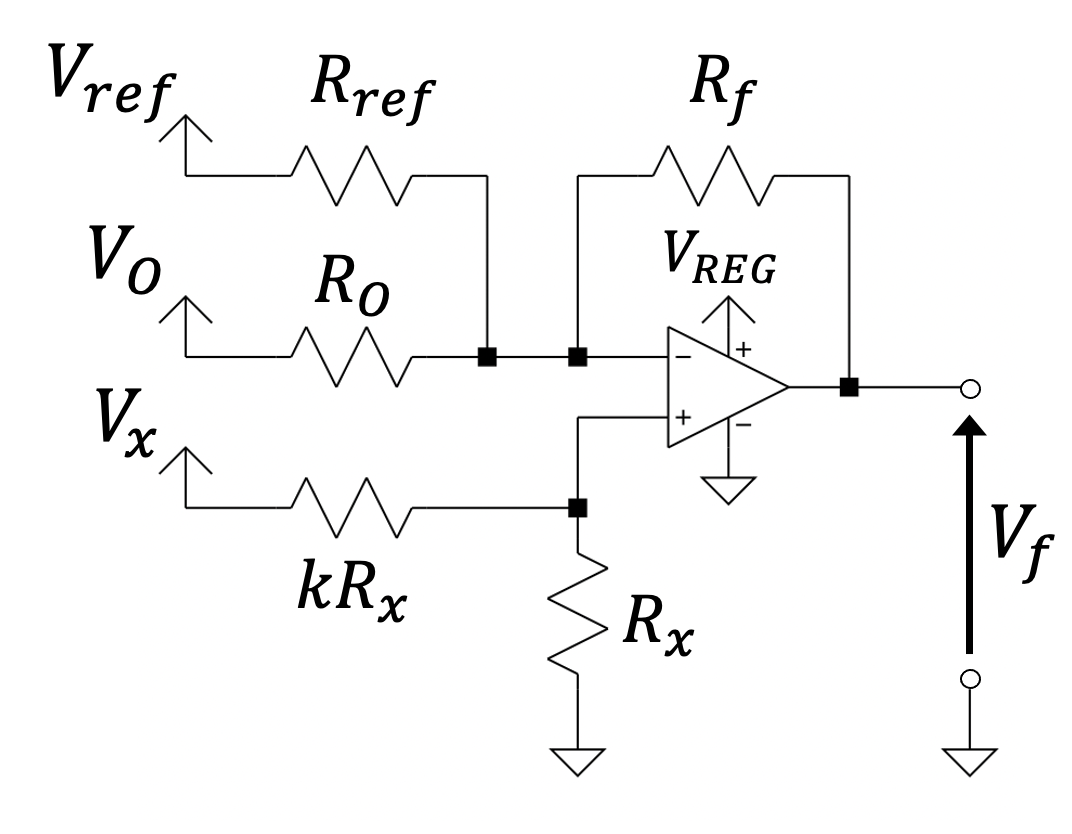
\includegraphics[scale=0.43]{img/circuito5.png}
  \caption{Lazo de corriente simplificado}
  \label{fig:Lazo de corriente simplificado}
\end{figure}

En este circuito, la salida puede hallarse por superposición. Eso da como resultado

\begin{equation}
    V_f = \left(1 + \frac{R_f}{R_{\text{ref}} \parallel R_O}\right)\frac{1}{k + 1} V_x-\frac{R_f}{R_{\text{ref}}} V_{\text{ref}} - \frac{R_f}{R_O}V_O. 
    \label{eq:salida sumador}
\end{equation}

Comparando las Ecuaciones \ref{eq:salida sumador} con \ref{eq:sumador} y junto con las Ecuaciones \ref{eq: formula de a}, \ref{eq:formula b} y \ref{eq:formula de c} puede concluirse que

\begin{minipage}{0.3\textwidth}
    \begin{equation}
    \left(1 + \frac{R_f}{R_{\text{ref}} \parallel R_O}\right)\frac{1}{k + 1} = 51
    \label{eq:entrada +}
    \end{equation}
\end{minipage}
\hfill
\begin{minipage}{0.3\textwidth}
    \begin{equation}
    \frac{R_f}{R_{\text{ref}}} = \frac{204}{25}
    \label{eq: entrada -1}
    \end{equation}
\end{minipage}
\hfill
\begin{minipage}{0.3\textwidth}
    \begin{equation}
    \frac{R_f}{R_O} = \frac{3111}{50}.
    \label{eq:entrada -2}
    \end{equation}
\end{minipage}

De esta forma, se tienen 3 ecuaciones con 4 incógnitas, por lo que hay un grado de libertad. Se elige $R_f = 10 \,\text{k} \Omega$. Posteriormente, de la Ecuación \ref{eq: entrada -1} se despeja $R_{\text{ref}} = 1,23 \,\text{k} \Omega$, de \ref{eq:entrada -2} se despeja $R_O = 160,7 \,\Omega$ y de \ref{eq:entrada +} se despeja $k = \frac{1019}{2550} \approx 0,4$. Dado que este circuito sí se va a implementar, es necesario elegir valores comerciales. Por tanto, se eligen $R_{\text{ref}} = 1,2 \,\text{k}\Omega$, $R_O = 150 \,\Omega$, $R_x = 10 \,\text{k} \Omega$ y $k  R_x = 3,9 \,\text{k} \Omega$.

\section{Simulaciones}

En esta sección se desarrollan las simulaciones efectuadas.

\subsection{Ganacia de Lazo}
\label{subsec: ganancia de lazo} 

\begin{figure}[H]
    \centering
    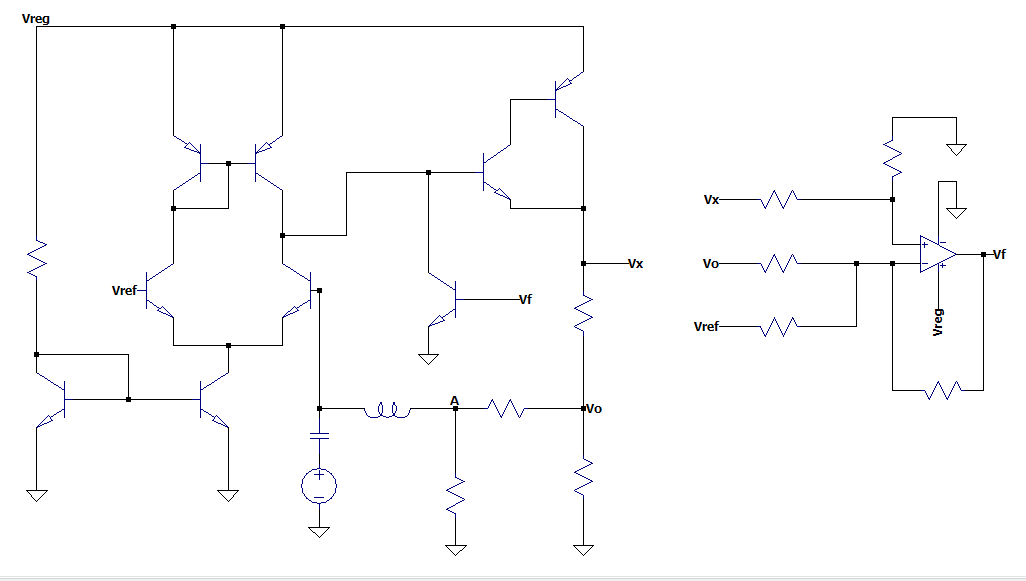
\includegraphics[width=0.7\linewidth]{img/Simulaciones/Circuito ganancia de Lazo.png}
    \caption{Circuito usado para simular la ganancia de lazo}
    \label{fig:circuito ganancia de lazo}
\end{figure}

Se utilizó el circuito de la \autoref{fig:circuito ganancia de lazo} para simular la ganancia de lazo. Se añaden el capacitor de $\SI{100}{\farad}$ y el inductor de $\SI{100}{\henry}$ para que la fuente de señal no afecte la polarización. De esta forma, se obtuvo el diagrama de Bode de la ganancia del lazo de tensión y corriente tomando la salida sobre el nodo A. Para ello, se seleccionaron valores de resistencia adecuados para cada lazo de realimentación, de modo que uno se active mientras el otro permanezca desactivado, y viceversa.

En la Figura \ref{fig:Bode} se muestra el bode del lazo de tensión para distintos valores de carga.

\begin{figure}[H]
    \centering
    
\includegraphics[width=0.85\linewidth]{img/Simulaciones/Bode.png}
    \caption{Diagrama de Bode del circuito con el lazo de tensión activo.}
    \label{fig:Bode}
\end{figure}

En este gráfico puede comprobarse que existe un rango de frecuencias medias en donde $|a\cdot f| = \SI{50}{\decibel}$, es decir, $|a\cdot f| \approx 316$. Esto justifica que $1 + a \cdot f \approx a \cdot f$, como se había asumido en la Ecuación \ref{eq:ganancia lazo cerrado}. Además, se observa que para estos valores de la carga el lazo de corriente todavía no está activado y, por lo tanto, la ganancia de lazo es prácticamente la misma para cualquier carga. 

En la Figura \ref{fig:bode corriente} se muestra el bode del lazo de corriente, donde se utilizo una carga de $R_L = 1\,\Omega$.

\begin{figure}[H]
    \centering
    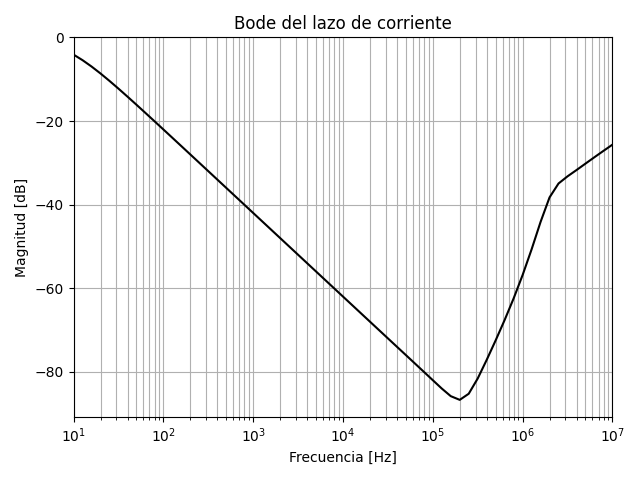
\includegraphics[width=0.7\linewidth]{img/Simulaciones/Bode corriente.png}
    \caption{Diagrama de Bode del circuito con el lazo de corriente activo.}
    \label{fig:bode corriente}
\end{figure}

Se observa que la ganancia es siempre menor a la unidad, lo que asegura que el circuito sea estable. 


\subsection{Regulación de línea y de carga}
\label{subsec:regulaciones}

Con los comandos de \textit{LTSpice} que se muestran en la Figura \ref{fig:comandos} se midieron las regulaciones de línea y de carga, representadas en las Figuras \ref{fig:RegLing grafico} y \ref{fig:RegCar grafico} respectivamente.

\begin{figure}[H]
    \centering
    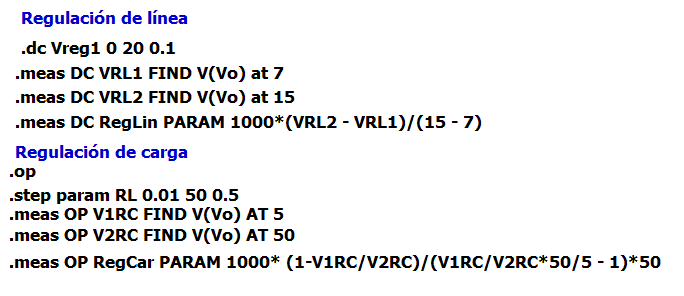
\includegraphics[scale=0.8]{img/Simulaciones/Comandos.png}
    \caption{Comandos de \textit{LTSpice}.}
    \label{fig:comandos}
\end{figure}

Cabe mencionar que la regulación de linea se midió con una carga constante $R_L = 50 \, \Omega$ y que la regulación de carga se midió con una tensión de entrada constante $V_{\text{REG}} = 9,5 \, \text{V}$.

\begin{figure}[H]
    \centering
    
\includegraphics[width=0.8\linewidth]{img/Simulaciones/Regulacion_de_Linea.png}
    \caption{Regulación de línea}
    \label{fig:RegLing grafico}
\end{figure}

Nótese que $V_\text{REG}^\text{min}\Big|_{V_O = 5\,\text{V}} = 6\,\text{V}$, por lo que se obtiene una tensión de \textit{dropout} de

\[
V_\text{drop} = V_\text{REG}^\text{min}\Big|_{V_O = 5\,\text{V}} - V_O = 1\,\text{V}.
\]

\begin{figure}[H]
    \centering
    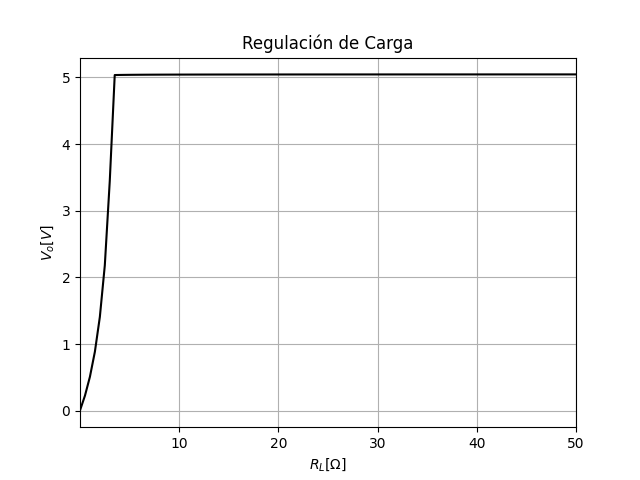
\includegraphics[width=0.8\linewidth]{img/Simulaciones/Regulacion_de_Carga.png}
    \caption{Regulación de carga}
    \label{fig:RegCar grafico}
\end{figure}

Las mediciones se vuelcan en el Cuadro \ref{tab:regulaciones}. 

\begin{table}[H]
\centering
\begin{tabular}{c c c}
\noalign{\hrule height 1pt} % Línea más gruesa aquí
Parámetro & Valor & Unidad \\
\hline
Regulación de línea & 8,41  & mV/V  \\
Regulación de carga & 7,07  & m$\Omega$  \\
\noalign{\hrule height 1pt} % Línea más gruesa aquí
\end{tabular}
\caption{Resultados de la medición}
\label{tab:regulaciones}
\end{table}

\subsection{Curva del \textit{foldback}}
\label{subsec:foldback}

Con los comandos \texttt{.step oct param RL 0.1 20 20} y \texttt{.op} se hizo un barrido para distintos valores de carga (similar a la sección anterior) para obtener la curva del \textit{foldback}, donde se grafican $V_O$ vs. $I_{R_L}$ y cuya gráfica se muestra en la Figura \ref{fig:Curva foldbakc}.

\begin{figure}[H]
    \centering
    
\includegraphics[width=0.8\linewidth]{img/Simulaciones/Curva_Foldback.png}
    \caption{Curva del \textit{foldback}}
    \label{fig:Curva foldbakc}
\end{figure}

De esta forma, se obtuvieron las características presentadas en el Cuadro \ref{tab:placeholder}.

\begin{table}[H]
    \centering
    \begin{tabular}{c c c}
    \noalign{\hrule height 1pt} % Línea más gruesa aquí
    Parámetro        & Valor especificado &Valor conseguido  \\
    \hline
    $I_{\text{MAX}}$ & 1,50 A              & 1,47 A                \\
    $I_{CC}$  & 0,400 A            & 0,401 A \\
    \noalign{\hrule height 1pt} % Línea más gruesa aquí
    \end{tabular}
    \caption{Características del \textit{foldback}}
    \label{tab:placeholder}
\end{table}


\subsection{Resumen de las características del circuito}

En el Cuadro \ref{tab:caracteristicas} se resumen los resultados de las Secciones \ref{subsec: ganancia de lazo}, \ref{subsec:regulaciones} y \ref{subsec:foldback}. Estos caracterizan al regulador diseñado. 

\begin{table}[H]
    \centering
    \begin{tabular}{c c c}
    \noalign{\hrule height 1pt} % Línea más gruesa aquí
    Parámetro & Valor & Unidad \\
    \hline
    Ganancia de lazo de tensión & 316 & - \\
    Regulación de línea & 8,41 & mV/V \\
    Regulación de carga & 7,07  & m$\Omega$ \\
    $I_{\text{MAX}}$ & 1,47  & A \\
    $I_{CC}$ &  0,401  & A \\
    \noalign{\hrule height 1pt} % Línea más gruesa aquí
    \end{tabular}
    \caption{Resumen de resultados}
    \label{tab:caracteristicas}
\end{table}

\newpage

\section{Diseño del Circuito Esquemático en Entorno CAD}

En esta fase del proyecto, se procedió a la captura del diseño lógico (se observa en la Figura \ref{fig:esquematico}) utilizando la herramienta \textit{KiCad EDA}. El objetivo central fue consolidar las etapas de control y potencia analizadas teóricamente en un esquema técnico normalizado, asegurando la integridad de los lazos de regulación y protección.

\begin{figure}[h]
    \centering
    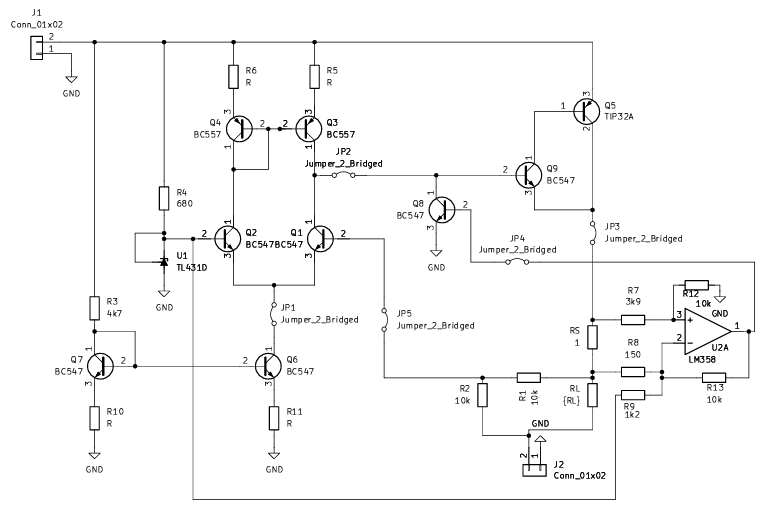
\includegraphics[width=1\linewidth]{img/esquematico.png}
    \caption{Esquemático realizado en la herramienta \textit{KiCad EDA} de la fuente regulada con protección de \textit{foldback}.}
    \label{fig:esquematico}
\end{figure}

El diseño de este esquemático se basó en el modelo SPICE (Figuras \ref{fig:Lazo de corriente 1} y \ref{fig:Lazo de corriente simplificado}), que  permitió optimizar la disposición de los componentes. Para garantizar el correcto funcionamiento, se tomó la decisión de incluir jumpers en lugares estratégicos, como en la salida del par diferencial, la retroalimentación de tensión, y el lazo de protección \textit{foldback} con el objetivo de verificar el adecuado desempeño del sistema de forma más práctica.

\subsection{Resumen de componentes}

En el diseño de la placa PCB, se utilizaron componentes clave para implementar las funciones de amplificación, regulación de tensión y protección por sobrecorriente. El Cuadro \ref{tab:componentes} resume los componentes a adquirir para la posterior implementación física del regulador.

\begin{table}[H]
\centering
\begin{tabular}{c c c}
\noalign{\hrule height 1pt} % Línea más gruesa aquí
Componente & Tipo & Cantidad \\ \hline

TBJ NPN & BC547 & 6 \\ 
TBJ PNP & BC557 & 2 \\ 
TBJ PNP & TIP32A & 1 \\ 

Referencia de tensión & TL431D & 1 \\ 
Amplificador operacional & LM358 & 1 \\ 

Resistor & 10k & 4 \\ 
Resistor & 4k7 & 1 \\ 
Resistor & 680 & 1 \\ 
Resistor & - & 4 \\ 
Resistor & 3k9 & 1 \\ 
Resistor & 150 & 1 \\ 
Resistor & 1k2 & 1 \\
Resistor & 1 & 1 \\

Conector & Bornera 2 pines & 2 \\ 
Jumper & Jumper 2.54 mm & 5 \\ 
\noalign{\hrule height 1pt} % Línea más gruesa aquí

\end{tabular}
\caption{Listado de componentes.}
\label{tab:componentes}
\end{table}

\section{Conclusiones}

En el presente trabajo se desarrolló el diseño de un regulador lineal tipo LDO, cumpliendo con las especificaciones establecidas en cuanto a tensión de salida, capacidad de corriente y comportamiento frente a perturbaciones. La arquitectura adoptada, basada en un amplificador diferencial junto con una etapa de salida tipo cuasi-darlington, permitió lograr una elevada ganancia a lazo abierto y un adecuado manejo de potencia, manteniendo un bajo valor de \textit{dropout}.

La implementación del lazo de realimentación de tensión resultó fundamental para reducir la fuerte dependencia de los parámetros del circuito respecto de la carga, mejorando significativamente la precisión y estabilidad de la tensión de salida. Asimismo, el diseño del lazo de corriente con característica \textit{foldback} permitió incorporar un mecanismo de protección eficaz frente a sobrecargas y cortocircuitos, limitando la corriente de manera controlada y reduciendo la disipación en condiciones críticas.

Los resultados obtenidos mediante simulación validan el diseño propuesto, evidenciando un alto valor de ganancia de lazo, junto con buenas prestaciones de regulación de línea y de carga, y una adecuada implementación de la curva de protección. En particular, los valores alcanzados para $I_\text{MAX}$ e $I_{CC}$ resultan consistentes con los objetivos planteados en las especificaciones de diseño.

Finalmente, este trabajo permitió integrar conceptos teóricos de electrónica analógica con herramientas de simulación y diseño, sentando una base sólida para la futura implementación física del sistema y su posterior validación experimental.

\newpage

\section{Bibliografía}

[1] P. R. Gray, P. J. Hurst, S. H. Lewis y R. G. Meyer, \textit{Analysis and Design of Analog Integrated Circuits}. Hoboken, NJ: Wiley, 5ta ed., 2009.

[2] STMicroelectronics, ``TIP32C: Power transistor.'', 2006.

[3] Texas Instruments, ``TL431, TL432: Precision Programmable Reference.'', 2025.

[4] ON Semiconductor, ``BC556B, BC557A, B, C, BC558B: Amplifier transistors (PNP Silicon).'', 2007.

[5] Fairchild Semiconductor, ``BC547, BC547A, BC547B, BC547C: NPN General Purpose Amplifier.'', 1997.
 
\newpage

\appendix

\clearpage
\vspace*{1cm}

\begin{center}
    {\Huge \textbf{Apéndices}}
\end{center}

\vspace{1cm}

\section{Demostración: alta influencia de la carga}

Se comienza calculando la ganancia a lazo abierto $a$ en modo diferencial. Para ello, se analizan las corrientes en el circuito de la
Figura \ref{fig:modo_diferencial}, suponiendo que todos los transistores están apareados y tienen el mismo $\beta$.

\begin{figure}[H]
  \centering
  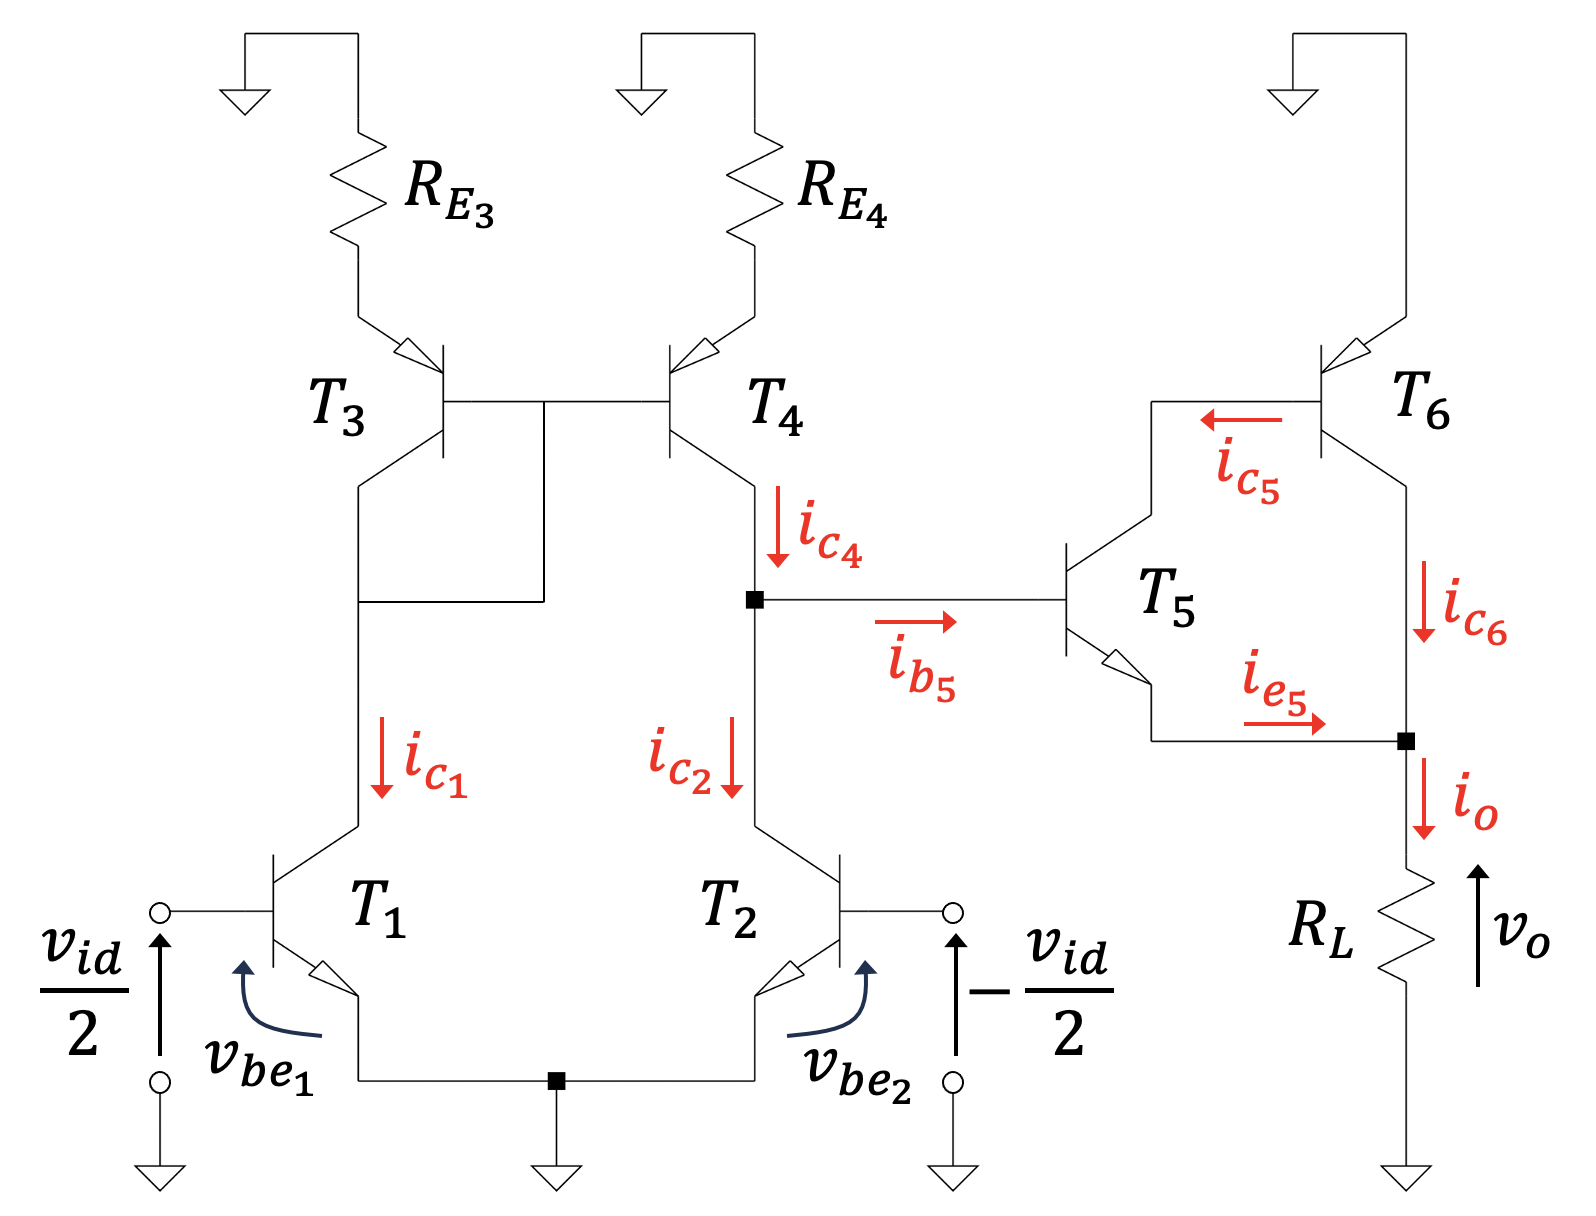
\includegraphics[scale=0.35]{img/modo_diferencial.png}
  \caption{Circuito a lazo abierto en modo diferencial.}
  \label{fig:modo_diferencial}
\end{figure}

Si $R_{E_3} = R_{E_4}$, el factor de copia de la fuente espejo PNP $T_3\text{-}T_4$ será $k_p = \beta / (\beta + 2)$. De este modo,
$i_{c_4} = k_p i_{c_1}$, lo que implica $i_{b_5} = k_p i_{c_1} - i_{c_2}$. De esto se sigue que $i_{c_5} = \beta(k_p i_{c_1} -
i_{c_2})$, $i_{e_5} = (\beta + 1)(k_p i_{c_1} - i_{c_2})$ y $i_{c_6} = \beta^2(k_p i_{c_1} - i_{c_2})$. Por tanto, se obtiene

\begin{equation}
i_o = (\beta^2 + \beta + 1)(k_p i_{c_1} - i_{c_2}).
\label{eq:io}
\end{equation}

Asimismo, se tiene 

\begin{align}
i_{c_1} = g_{m_1} v_{{be}_1} = g_{m_1}\frac{v_{id}}{2}, \quad & \label{eq:ic1} \\
i_{c_2} = g_{m_2} v_{{be}_2} = -g_{m_2}\frac{v_{id}}{2}, \quad & \label{eq:ic2}
\end{align}

y como $i_{c_1} = -i_{c_2}$ entonces $g_{m_1} = g_{m_2} = I_{C_1} / V_\text{th}$.

Finalmente, reemplazando las Ecuaciones \ref{eq:ic1} y \ref{eq:ic2} en la Ecuación \ref{eq:io} se obtiene

\begin{align}
a &= \left.\frac{v_o}{v_{id}}\right|_{v_{ic}=0} = \frac{i_o R_L}{v_{id}} \notag \\
  &= (\beta^2 + \beta + 1)(1 + k_p)\frac{I_{C_1} R_L}{2 V_\text{th}}.
\label{eq:ganancia}
\end{align}

\begin{figure}[H]
  \centering
  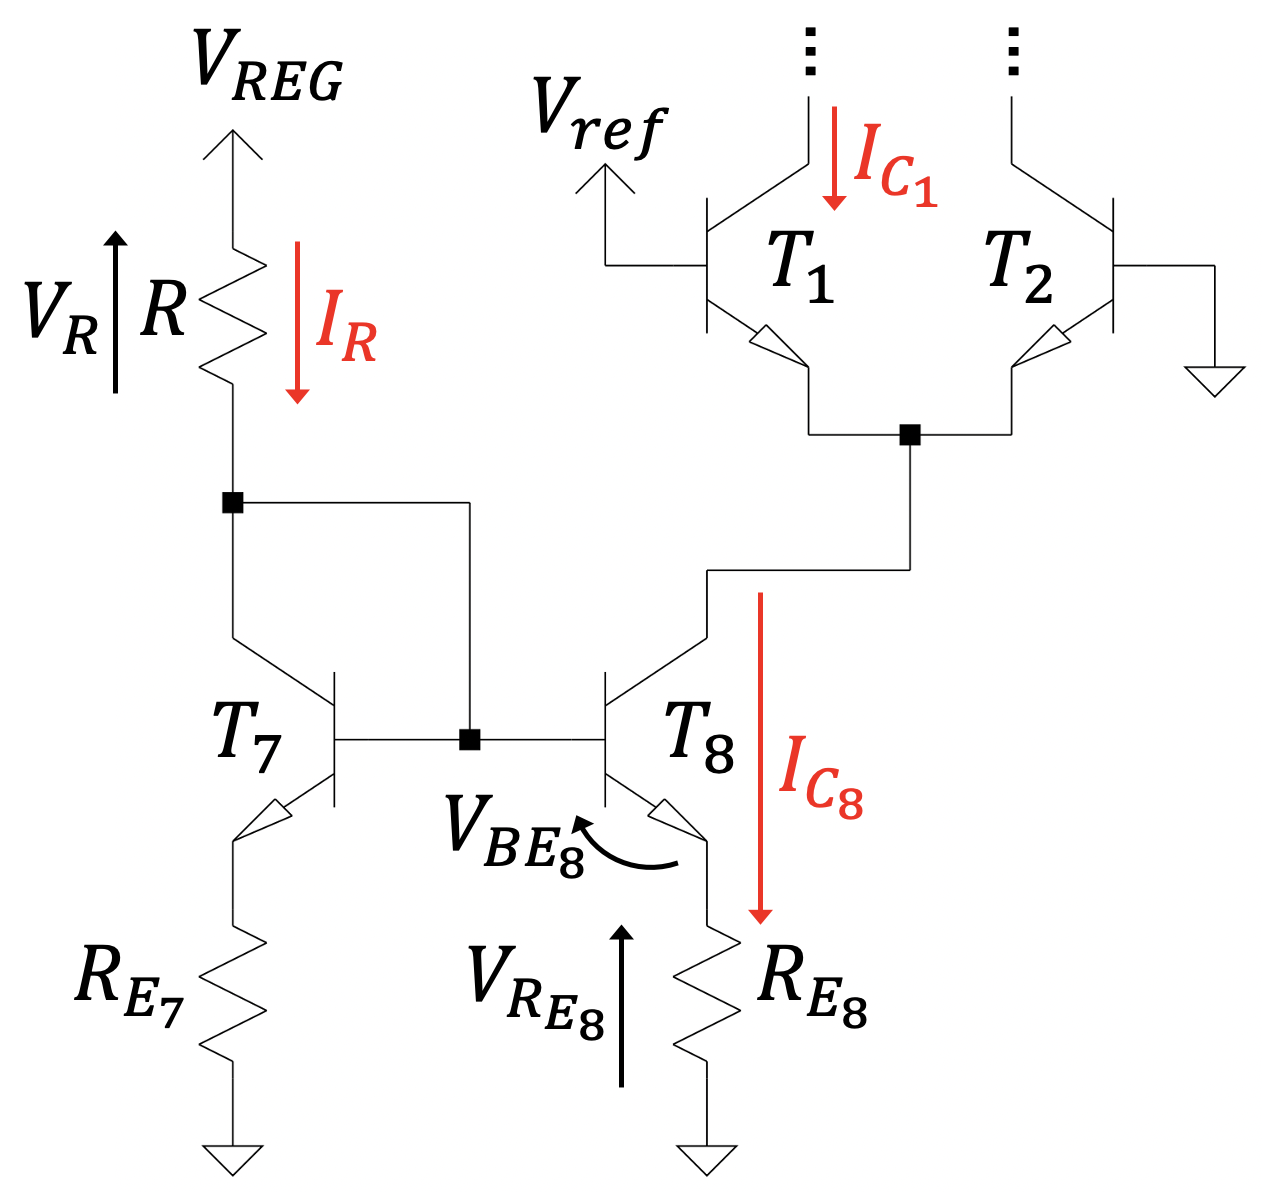
\includegraphics[scale=0.25]{img/continua.png}
  \caption{Porción del circuito de polarización.}
  \label{fig:continua}
\end{figure}

Siendo un valor típico para estos transistores $\beta = 290$, la tensión térmica $V_\text{th} = 25,7$ mV y para una ganancia $a =
50\,000$, despejando en la Ecuación \ref{eq:ganancia} se obtiene que $I_{C_1}(R_L) = 15,3~\text{mV} / R_L$. Como $I_{C_8} = 2I_{C_1}$,
se tiene que $I_{C_8}(R_L) = 30,6~\text{mV} / R_L$ ---véase Figura \ref{fig:continua}---.

Si $R_{E_7} = R_{E_8}$, el factor de copia de la fuente espejo NPN $T_7\text{-}T_8$ será $k_n = \beta / (\beta + 2)$. De este modo,
$I_R = I_{C_8} / k_n$, por lo que $I_R(R_L) = 30,8~\text{mV} / R_L$. Además, $V_{R_{E_8}} = I_{C_8} R_{E_8}$ por lo que
$V_{R_{E_8}}(R_L) = 30,6~\text{mV} \cdot (R_{E_8} / R_L)$.

Por tanto, 

\[
R(R_L) = \frac{V_R(R_L)}{I_R(R_L)} = \frac{V_\text{REG} - V_{R_{E_8}}(R_L) - V_{{BE}_8}}{I_R(R_L)} \approx 286 R_L - R_{E_8}.
\]

La resistencia de polarización $R$ depende linealmente de la carga $R_L$ y con una pendiente muy elevada; por lo que, ante cualquier
mínima variación en la carga, el valor de $R$ variará muchísimo, como se muestra en la Figura \ref{fig:lineal}. Esto demuestra que se
requiere un circuito realimentado para eliminar la alta dependencia de la carga en los parámetros diseñados.

\begin{figure}[H]
  \centering
  
\includegraphics[scale=0.3]{img/lineal.png}
  \caption{Gráfico de $R$ vs. $R_L$.}
  \label{fig:lineal}
\end{figure}

\section{Demostración: \textit{foldback}}

Dado el siguiente sistema de ecuaciones

\[
\begin{cases}
V_S = \frac{R_4}{R_3}R_S I_O \\
V_\text{ref-C} = \alpha V_\text{ref} + \beta V_O \\
V_f = \frac{R_6}{R_5}(V_S - V_\text{ref-C}) \\
V_S = V_x - V_O
\end{cases}
\]

es posible escribir a $V_f$ como combinación lineal del resto de las tensiones.

\begin{align*} 
V_f &= \underbrace{\frac{R_6}{R_5}\frac{R_4}{R_3}}_a \,R_S I_O\ \underbrace{-\ \frac{R_6}{R_5}\alpha}_b \, V_\text{ref} \ \underbrace{-\ \frac{R_6}{R_5}\beta}_{c'} \, V_O \\
&= a \, V_s + b \, V_\text{ref} + c' \, V_O \\
&= a \, V_x + b \, V_\text{ref} + \underbrace{(c' - a)}_c \, V_O \\
&= a \, V_x + b \, V_\text{ref} + c \, V_O
\end{align*}

Por tanto, se obtiene lo siguiente.

\[
\begin{cases}
    a = \frac{R_6}{R_5}\frac{R_4}{R_3} \\
    b = -\frac{R_6}{R_5}\alpha \\
    c = -\frac{R_6}{R_5}\left(\beta + \frac{R_4}{R_3}\right)
\end{cases}
\]

\end{document}